% !TeX root = main.tex
% \section{Homological Sensor Networks and the TCC} % (fold)
% \label{sec:tcc}

We first implemented the Topological Coverage Criterion (TCC), detailed below, then modified it to conduct experiments on the efficacy of trajectories of persistence diagrams.

\subsection{The Topological Coverage Criterion}

To recap, we have an unknown, bounded domain $\D$ with boundary $\B$ and a finite collection of sample points $P\subset\D$.
Each sensor, represented by a single point $p\in P$, can do the following:

\vspace{3ex}
\begin{center}
\setlength{\fboxsep}{2ex}
\fbox{\parbox{\textwidth}{
\begin{small}
\textbf{Sensor Capabilities}
    \begin{itemize}
        \item[a.]\textbf{(Communication Radii)} detect the presence, but not location or distance, of sensors within distances $\alpha > 0$ and $\beta \geq 3\alpha$, and discriminate between sensors within each scale,
        \item[b.]\textbf{(Coverage Radius)} cover a radially symmetric subset of the domain with radius $\alpha$,
        \item[c.]\textbf{(Boundary Detection)} detect the presence of the boundary $\B$ within distance $\alpha$.
    \end{itemize}
\end{small}
}}\end{center}\vspace{3ex}

\begin{definition}
    For a pair of sets $(\D, \B)$ such that $\B\subseteq \D$, we say that $\B$ \emph{surrounds} $\D$ if there is no path from $\D\setminus\B$ to $\comp{\D}$ that does not intersect $\B$.
    Formally, $\B$ surrounds $\D$ if and only if $H_0(\D\setminus \B) \cong H_0(\comp{\B}, \comp{\D})$, where $\comp{\D}$ denotes the complement of $\D$ in the ambient space containing $\D$.
\end{definition}

If such a pair satisfies the following conditions for $0 < 3\alpha\leq \beta$, we want to certify that a finite sample $P\subset\D$ covers $\D$ at scale $\alpha$ in the sense that $\D\setminus\B^{2\alpha}\subset P^\alpha$.
\euclidean{Although the TCC holds for more general spaces with a few technical assumptions (see~\cite{cavanna17when}) we will assume that our domain $\D$ is a subset of $\R^d$ for the sake of simplicity.}

\vspace{2ex}
\begin{center}
\setlength{\fboxsep}{2ex}
\fbox{\parbox{\textwidth}{
% \vspace{1ex}\hspace{1ex}
\textbf{Geometric Assumptions}
\begin{small}
    \begin{enumerate}
    \setcounter{enumi}{-1}
        \item \textbf{(Domain)} \noeuclidean{$\D$ is a bounded, compact length space homeomorphic to a subset of $\R^d$}\euclidean{$\D$ is a bounded, compact subset of $\R^d$} and $\B\subseteq \D$ is closed and surrounds $\D$.
        \item \textbf{(Components are not too small)} $\hom_0(\D\setminus\B^{\alpha+\beta}\hookrightarrow \D\setminus\B^{2\alpha})$ is surjective.
        \item \textbf{(Components are not too close)} $\hom_0(\D\setminus\B^{2\alpha}\hookrightarrow (\D\setminus \B)^{2\alpha})$ is injective.
    \end{enumerate}
\end{small}
}}\end{center}\vspace{4ex}

% Lemma~\ref{lem:shrunken_to_relative} allows us talk about the homology of a subset of the domain $\D\setminus\B^\e$ in terms of relative homology.
% \begin{lemma}\label{lem:shrunken_to_relative}
%     If $\B$ surrounds $\D$, then for all $\e>0$, $\hom_0((\D\setminus\B^{\e},\emptyset)\hookrightarrow (\comp{\B^{\e}},\comp{\D^{\e}}))$ is an isomorphism.
% \end{lemma}

\figblock{%
\begin{wrapfigure}{r}{0.5\linewidth}%
    \centering
    \vspace{-5ex}
    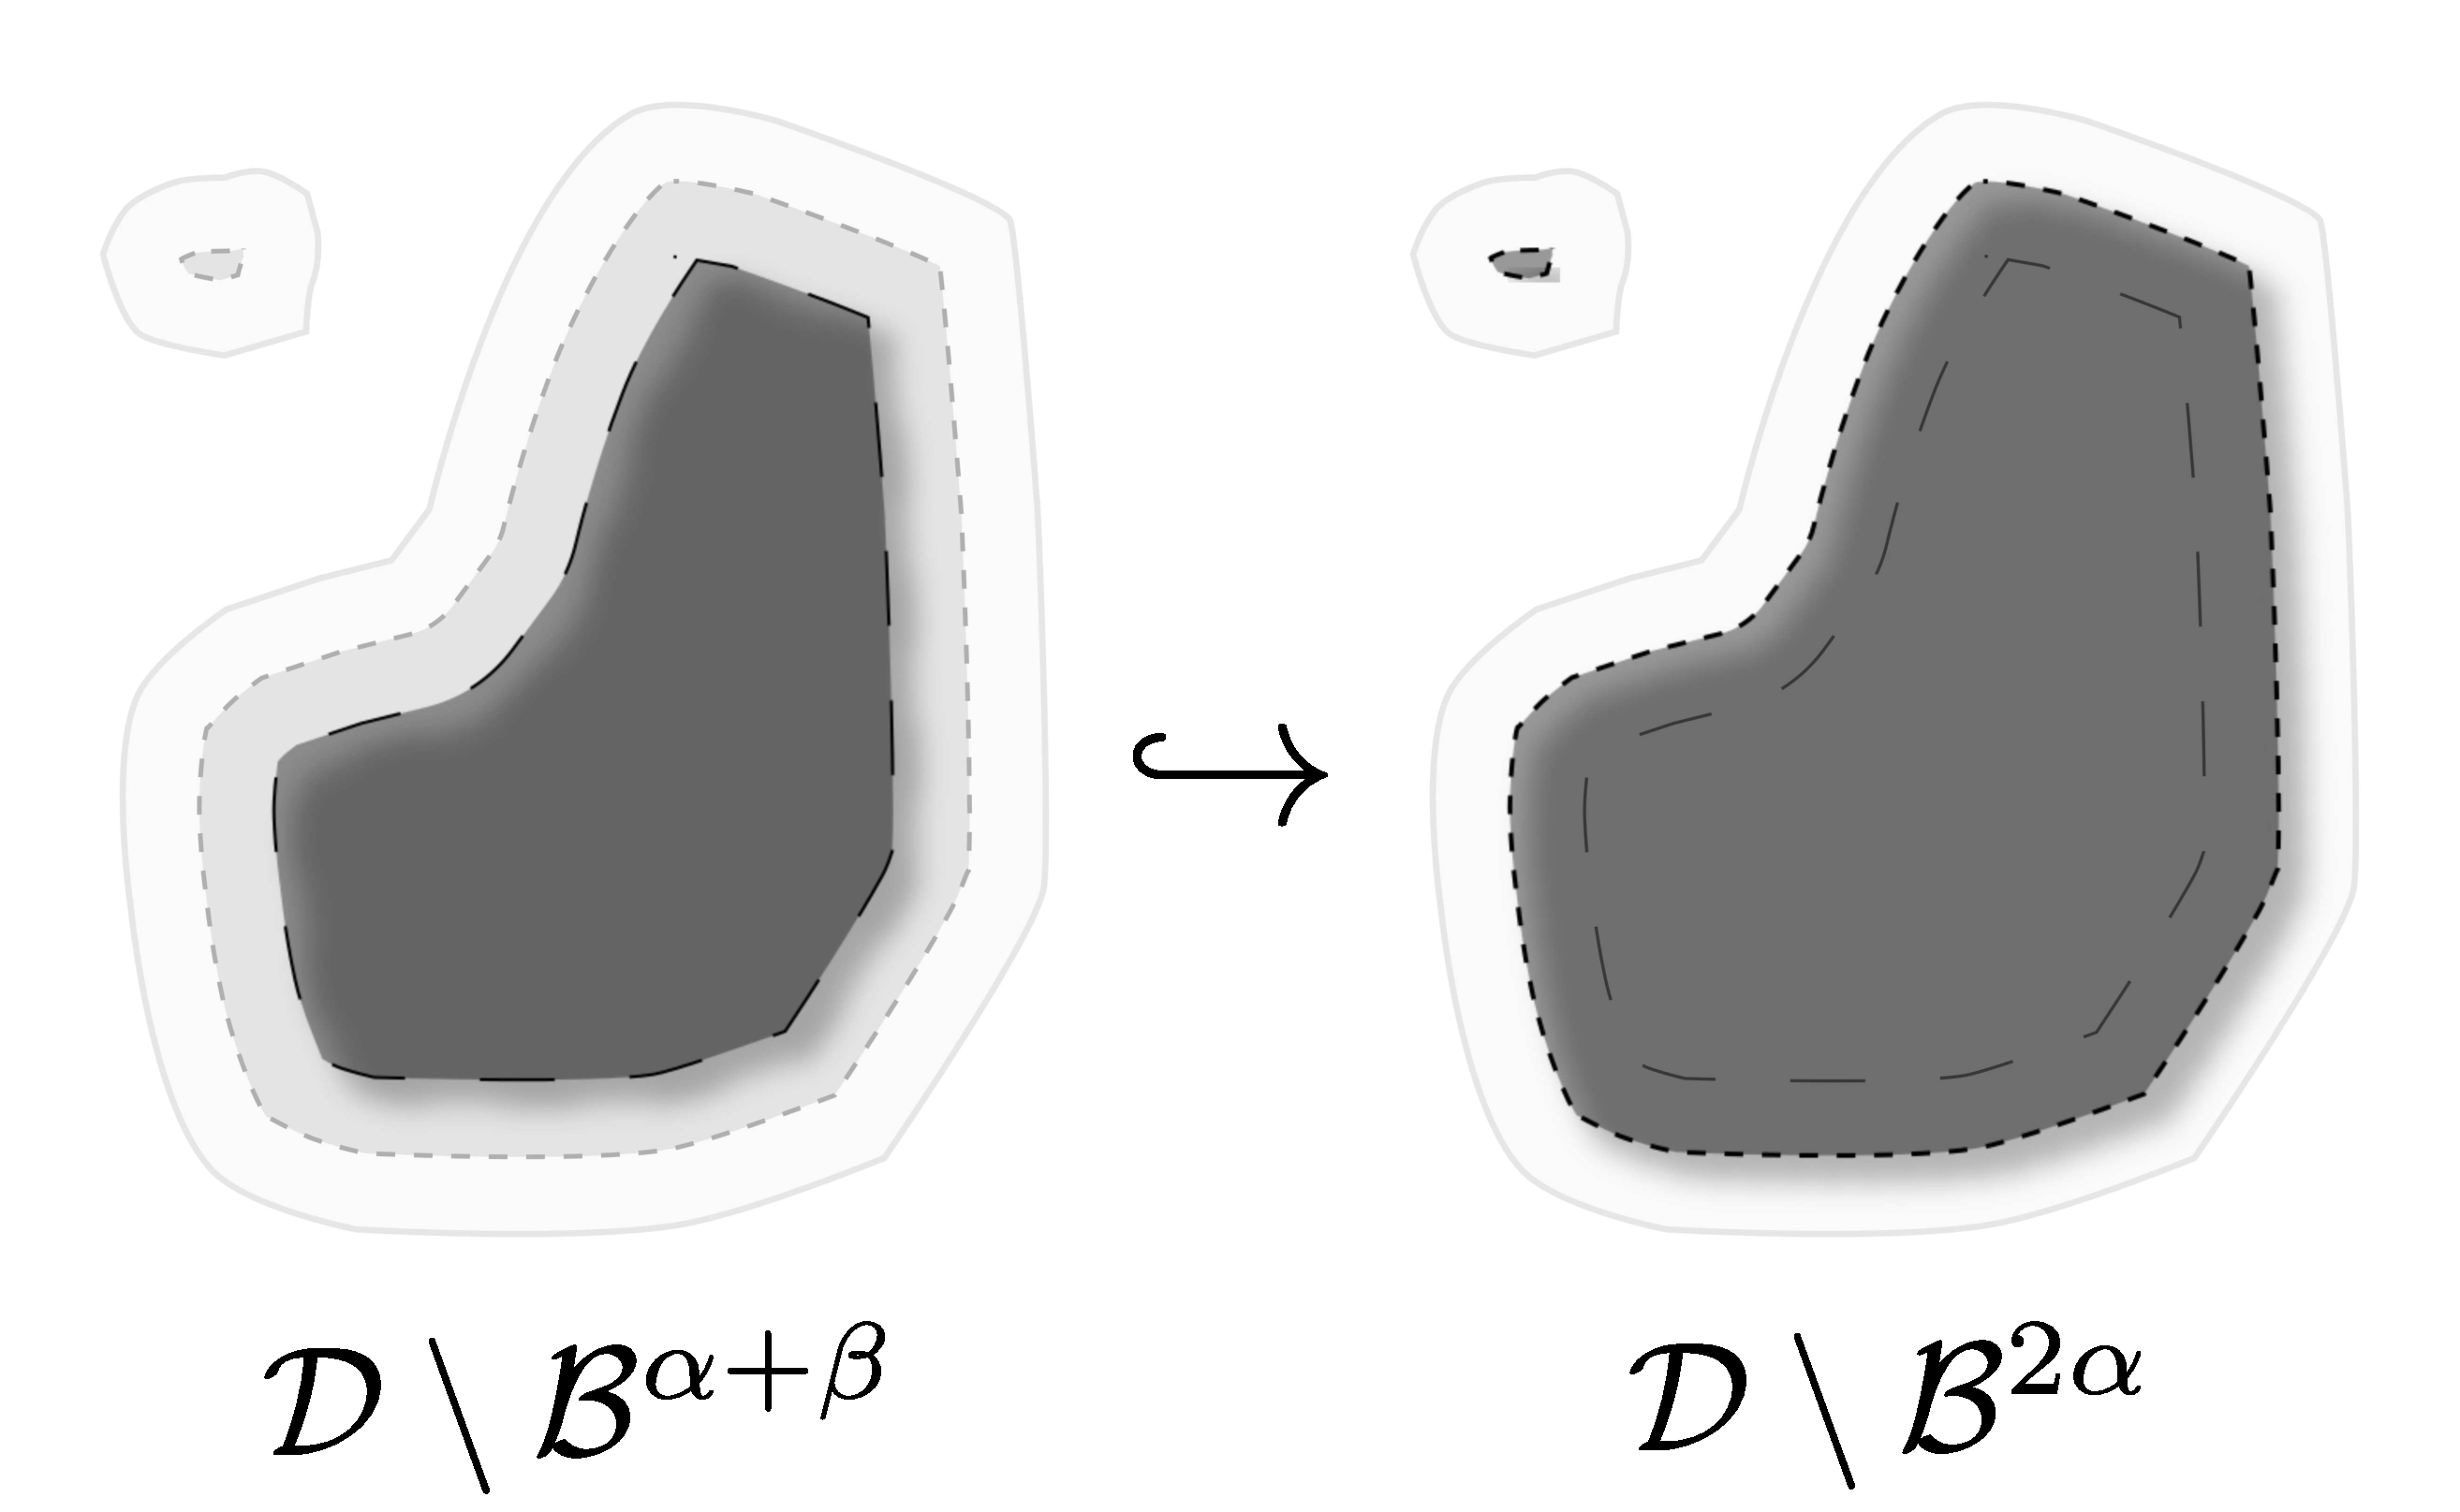
\includegraphics[scale=0.15]{figures/a1_composite.eps}
    \caption{A domain that violates Assumption $1$ as the upper-left component appears in the inclusion from $\D\setminus\B^{\alpha+\beta}$ to $\D\setminus\B^{2\alpha}$.}
    \label{fig:assumption1}
\end{wrapfigure}}

Assumption~1 disallows domains with components that are too small to be included in the map from $\D\setminus\B^{\alpha+\beta}\hookrightarrow\D\setminus\B^{2\alpha}$ so we can reliably compare the coverage region to the sampled subset of the domain in terms of the $0$-dimensional homology, or connected components.
Fig.~\ref{fig:assumption1} illustrates a domain in which the induced map is not surjective.

Assumption $2$ requires that the components of $\D\setminus\B^{2\alpha}$ are spaced out well enough so that no components are joined with inclusion into $\D^{2\alpha}$.
This includes regions of a connected component of $\D$ that are ``pinched'' into two in $\D\setminus\B^{2\alpha}$ as well as pairs of components in $\D$ that are too close.
Both are illustrated in Fig.~\ref{fig:assumption2}.
% Fig.~\ref{fig:assumption2} illustrates domains which violate Assumption $2$.

% \vspace{2ex}
\figblock{%
\begin{figure}[htbp]
    \centering
    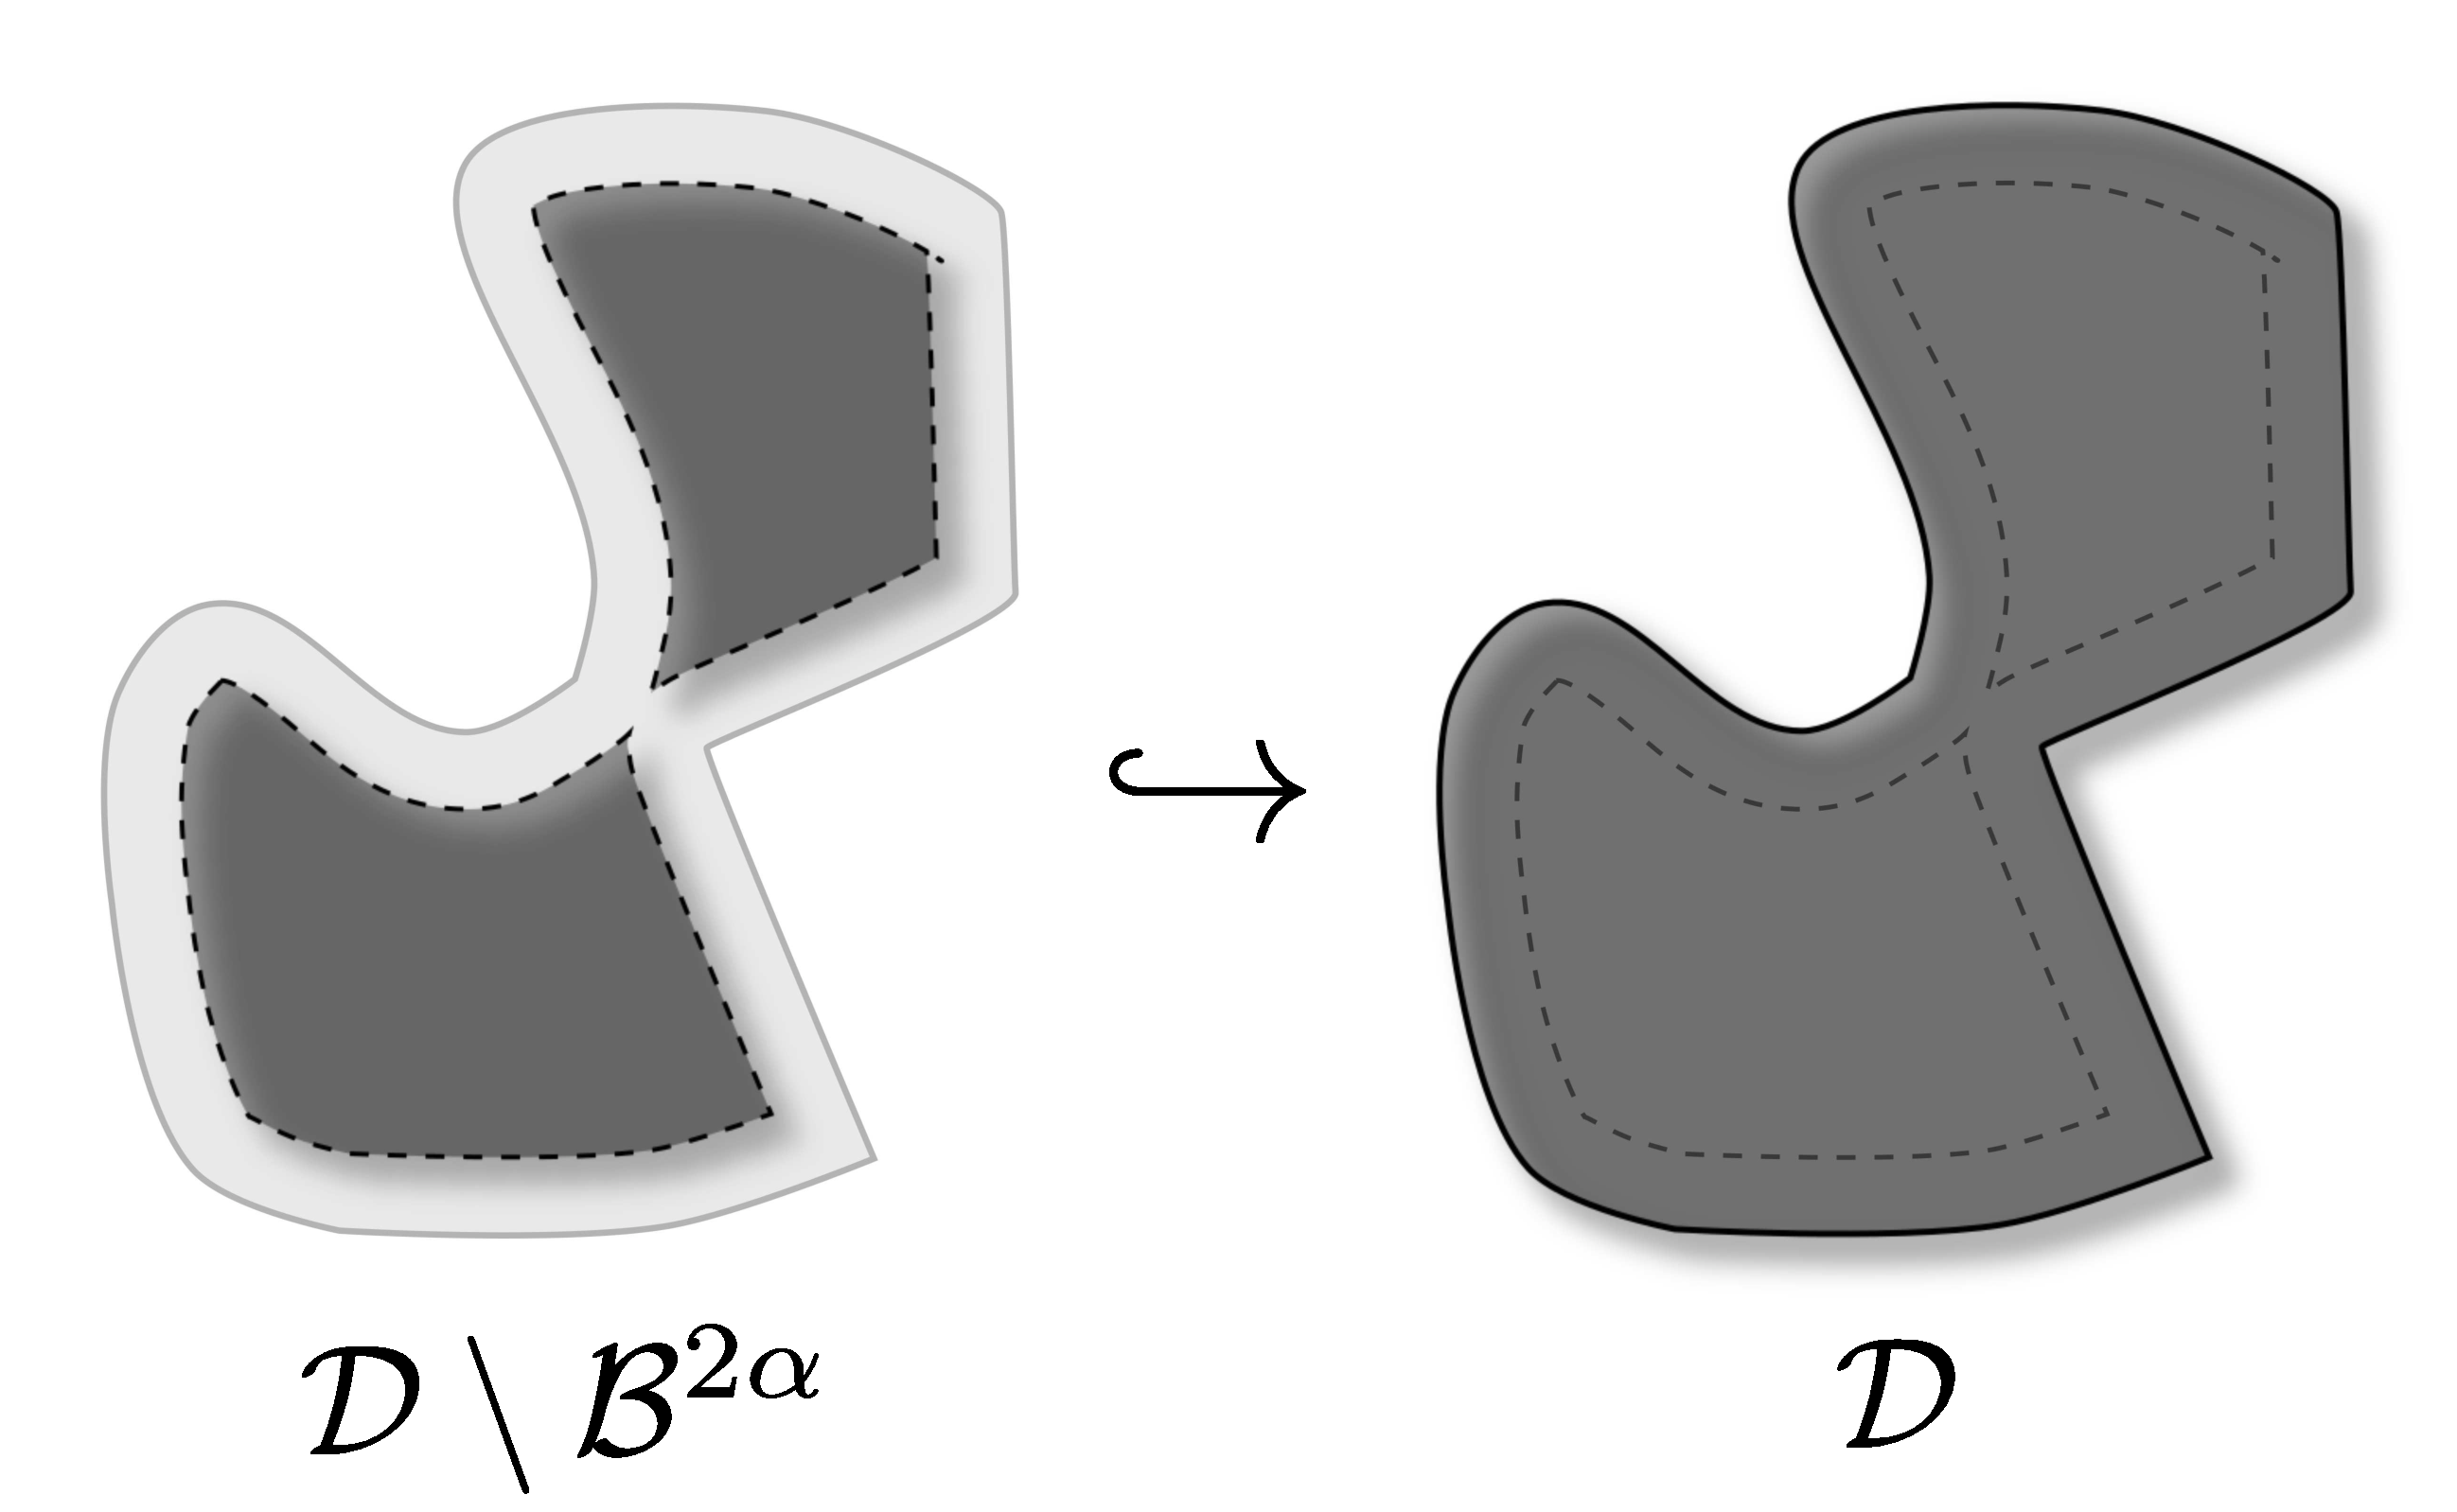
\includegraphics[scale=0.14]{figures/a2_2_composite.eps}\hspace{5ex}
    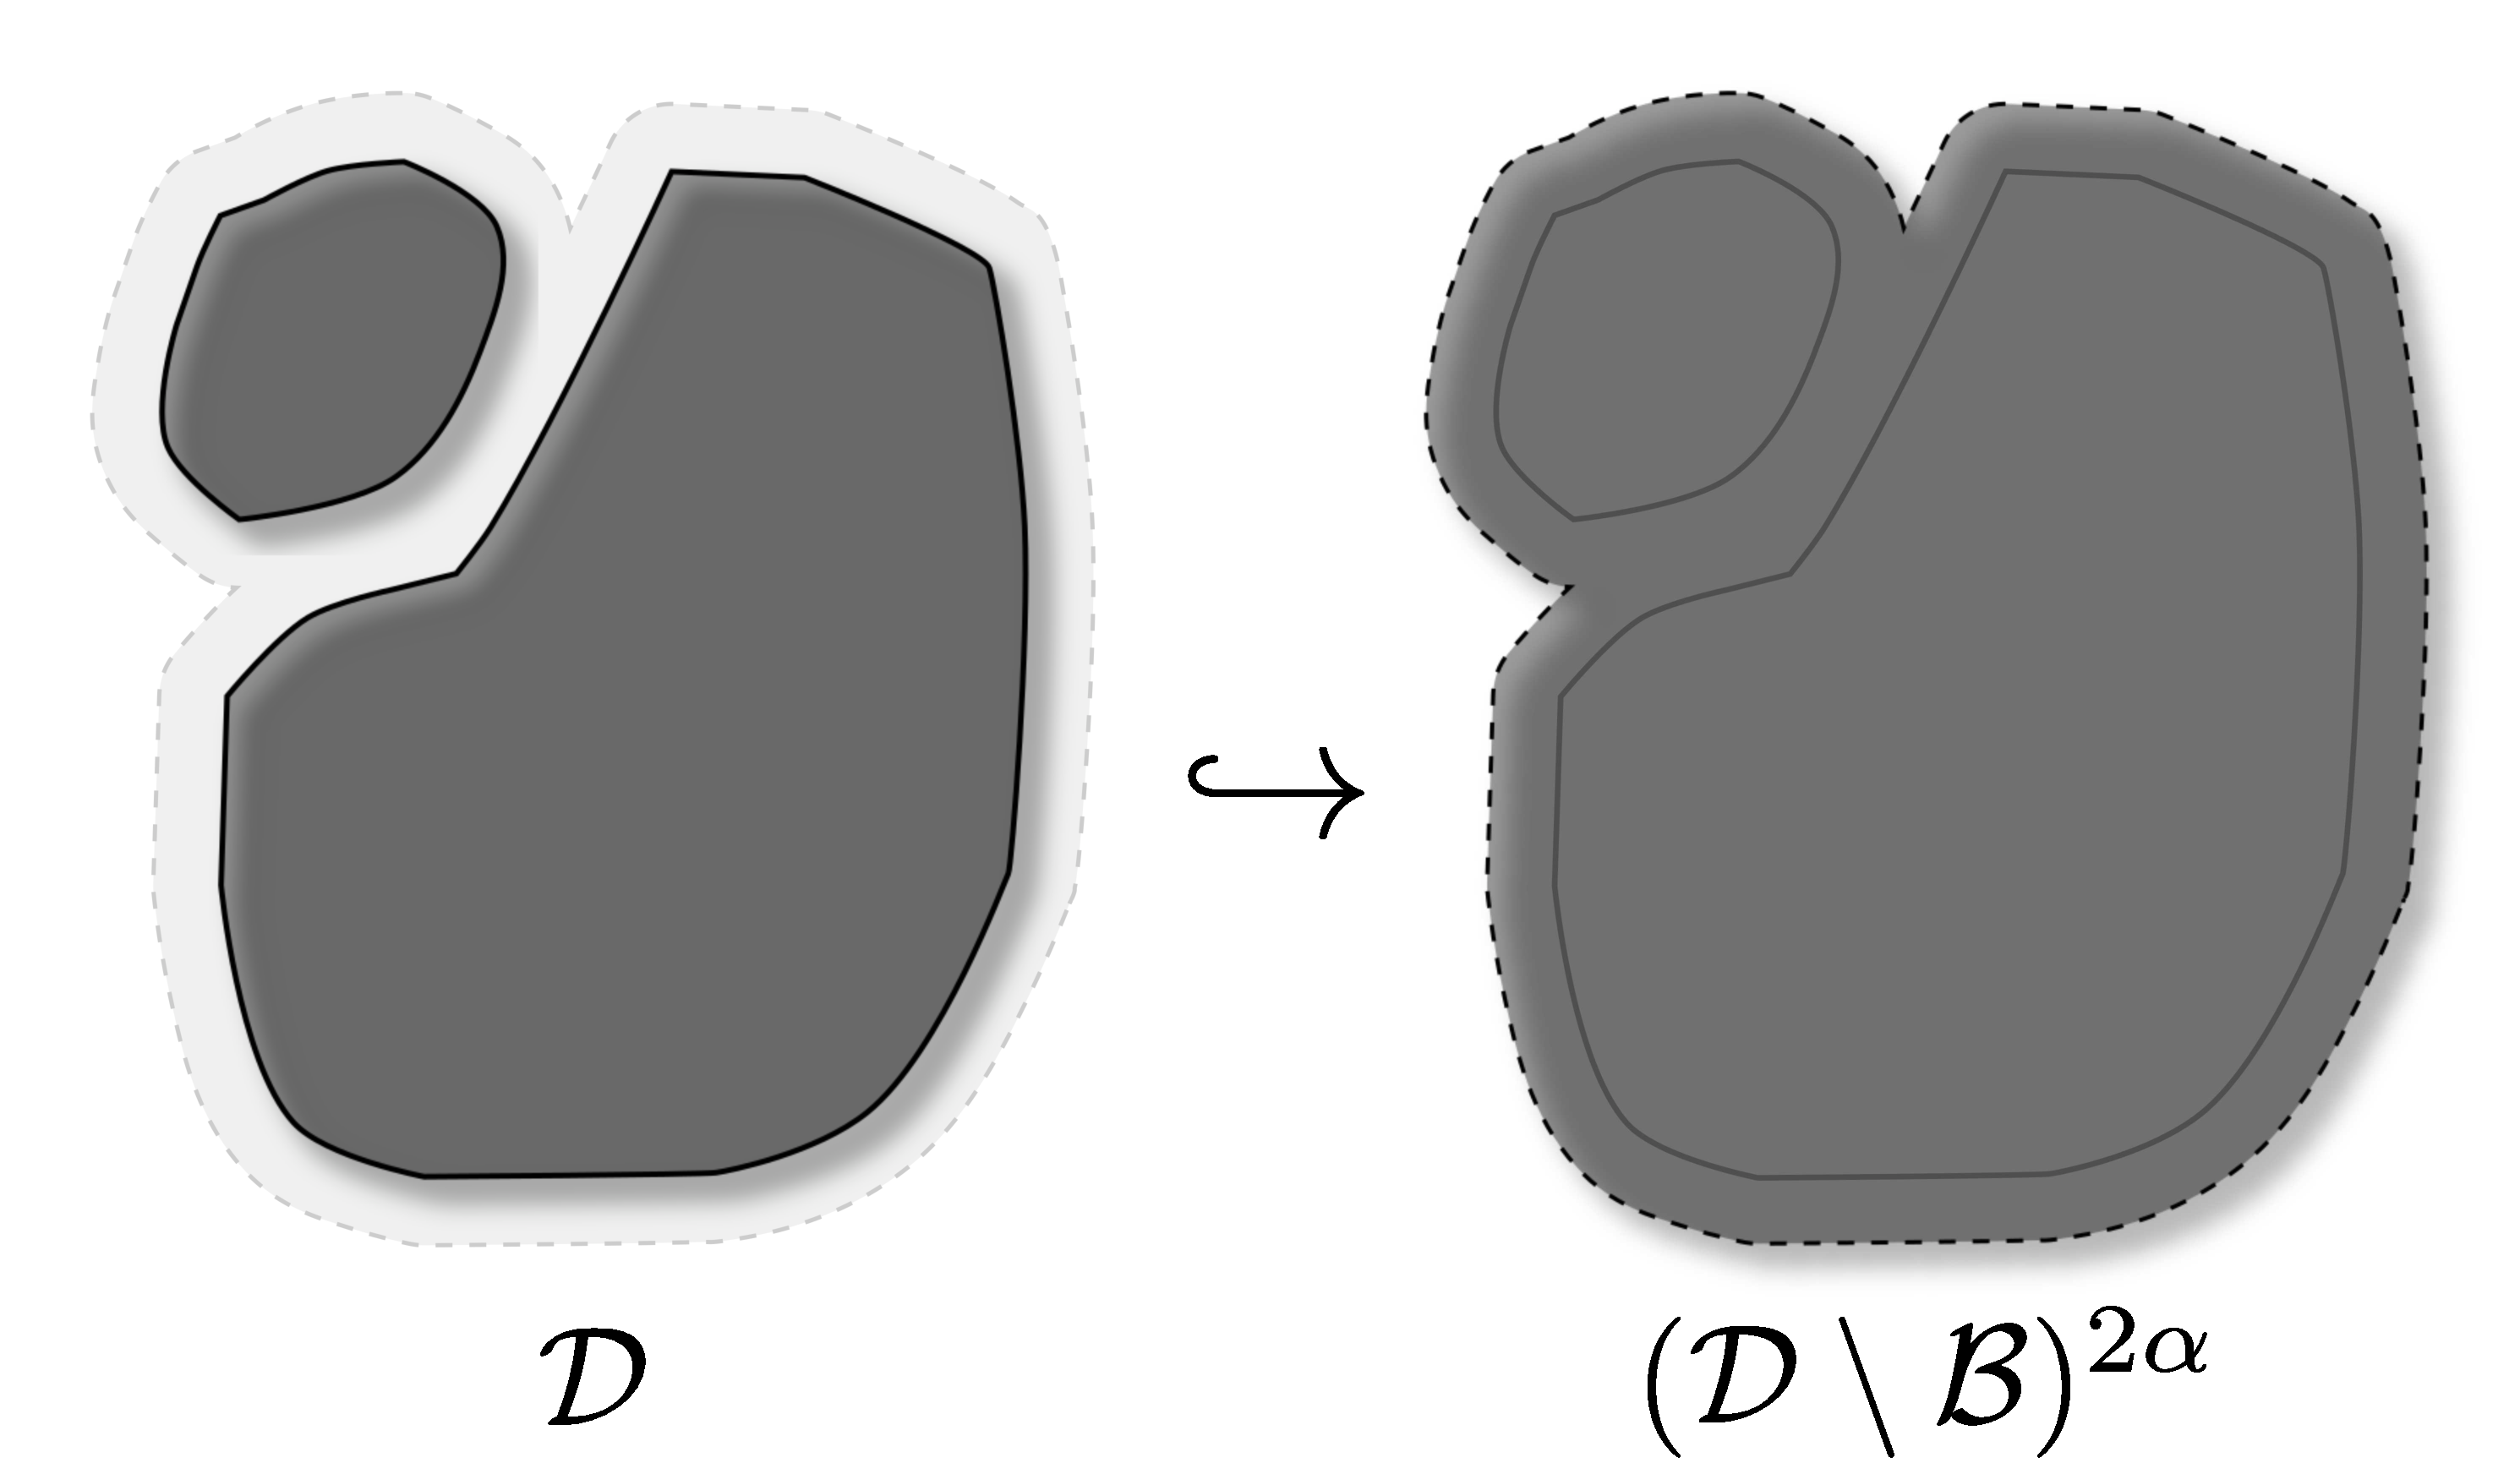
\includegraphics[scale=0.14]{figures/a2_1_composite.eps}
    \caption{Domains which violate Assumption 2 in which components are lost in the inclusions $\D\setminus\B^{2\alpha}\hookrightarrow \D$ and $\D\hookrightarrow (\D\setminus \B)^{2\alpha}$ respectively. In the first case a single component is pinched apart in $\D\setminus\B^{2\alpha}$. In the second, two components which are too close are merged in $(\D\setminus \B)^{2\alpha}$.}
    \label{fig:assumption2}
\end{figure}}

Assumptions 0-2 are necessary in order to prove the Geometric TCC (see~\cite{cavanna17when}) and, in particular, Assumption $2$ is necessary for the Algorithmic TCC (Theorem~\ref{thm:algorithmic_tcc}) in order to bound the number of connected components of the shrunken domain $\D\setminus\B^{2\alpha}$.

\subsubsection{Algorithmic TCC}

% Given a graph $G = (V, E)$ a \textbf{clique} is a collection of vertices $\sigma\subseteq V$ such that $\{u,v\}\in E$ for all $u,v\in\sigma$.
% \begin{definition}
%     The \textbf{clique complex} of $G$ is defined to be a simplicial complex with simplices for each clique in $G$.
%     \[ \clique(G) := \{ \sigma\subseteq V\mid \forall u,v\in\sigma, \{u,v\}\in E \}. \]
%
%     Given a pair of graphs $(G, H)$ where $H$ is a subgraph of $G$, we will denote the pair of Clique complexes as $\clique(G,H) = (\clique(G),\clique(H))$.
% \end{definition}

Let $(\D,\B)$ be a pair of spaces satisfying Assumptions $0$--$2$ for constants $\alpha > 0$, $\beta\geq 3\alpha$.
The input to Algorithm~\ref{alg:rips_certify_coverage} will be a collection of sensors $P\subset\D$ with the capabilities defined above where $Q = \{ p\in P\mid \ball_\alpha(p)\cap \B\neq\emptyset \}$.

% pair of graphs $(G_1, G_2)$, a finite weighted point sample $P\subset \D$ and a subsample $Q=\{p\in P\mid \ball_\alpha(p)\cap\B \neq \emptyset\}$.

% \vspace{2ex}
% \begin{center}
% \setlength{\fboxsep}{2ex}
% \fbox{\parbox{0.75\textwidth}{
% % \vspace{1ex}\hspace{1ex}
% \textbf{Input Assumptions}
%     \begin{enumerate}
%     \setcounter{enumi}{+2}
%         \item The graphs $G_1, G_2$ have a vertex set $P\subset\D$ and subgraphs $G_1[Q], G_2[Q]$ induced by restriction to the vertex set
%         \[Q = \{ p\in P\mid \ball_\alpha(p)\cap \B\neq\emptyset \}.\]
%         \noeuclidean{\item $\U = \{\ball_\e(p)\mid p\in P\}$ is a good cover for $\e\in\{\alpha,\beta\}$.}
%         \kcoverage{\item $\clique_k(G_1)\subseteq\cech_k^\alpha(P)\subseteq\cech_k^\beta(P)\subseteq\clique_k(G_2)$.}
%         \nokcoverage{\item $\clique(G_1)\subseteq\cech^\alpha(P)\subseteq\cech^\beta(P)\subseteq\clique(G_2)$.}
%         \item Each component of $\D\setminus\B^{2\alpha}$ contains a point in $P$.
%         \noeuclidean{\kcoverage{\item There exists a triangulation $\K$ of $\R^d\cup\{\infty\}$ and triangulations of $P_k^\e$ and $Q_k^\e$, $L_\e$ and $M_\e$ respectively, where $M_\e\subset L_\e$ in $\K$, for $\e\in\{\alpha,\beta\}$.}
%         \nokcoverage{\item There exists a triangulation $\K$ of $\R^d\cup\{\infty\}$ and triangulations of $P^\e$ and $Q^\e$, $L_\e$ and $M_\e$ respectively, where $M_\e\subset L_\e$ in $\K$, for $\e\in\{\alpha,\beta\}$.}}
%     \end{enumerate}
% }}\end{center}\vspace{3ex}
%
% The input graphs will be used to construct clique complexes, which by Assumption $5$ can be interleaved with \v Cech complexes at scale $\alpha$ and $\beta$.
% % \euclidean{The input graphs will be used to construct Rips complexes which can be interleaved with \v Cech complexes by equation~\ref{eq:jung_inclusion}.}
% \noeuclidean{Assumption $4$ allows us to apply the Persistent Nerve Lemma~\cite{chazal08towards}.
% Note that Assumption $5$ is satisfied when every clique $\sigma\subseteq G_1$ satisfies $\bigcap_{v\in\sigma} \ball_\alpha(v)\neq \emptyset$ and $\ball_\beta(u)\cap\ball_\beta(v)\neq\emptyset$ implies $\{u,v\}\in E(G_2)$ for all $u, v\in\sigma$.
% When the domain $\D$ is equipped with the Euclidean metric, Assumption $5$ is equivalent to the interleaving provided by Jung's theorem (Equation~\ref{eq:jung_inclusion}) where the \kcoverage{$k$-clique complex of $G_1$ can be taken as the $k$-Rips}\nokcoverage{clique complex of $G_1$ can be taken as the Rips} complex of $P$ at scale $\alpha/\jungd$.}
% \euclidean{Note that because we have assumed our domain $\D$ is equipped with the Euclidean metric Assumption $4$ is equivalent to the interleaving provided by Jung's theorem (Equation~\ref{eq:jung_inclusion}) where the \kcoverage{$k$-clique complex of $G_1$ can be taken as the $k$-Rips}\nokcoverage{clique complex of $G_1$ can be taken as the Rips} complex of $P$ at scale $\alpha/\jungd$.}
% \noeuclidean{Finally, }Assumption \noeuclidean{6}\euclidean{5} is required to prove a bound on the number of connected components of $\D\setminus\B^{2\alpha}$ using a computable combinatorial structure.

% \begin{theorem}[Geometric TCC]\label{thm:geometric_tcc}
%   Given a compact, locally contractible domain $\D\subset\R^d$ with boundary $\B\subset\D$, a sample $P\subset\D$, $Q = \B^\alpha\cap P$ and $i_*:\hom_0(\comp{Q^{\beta}},\comp{P^{\beta}})\to\hom_0(\comp{Q^{\alpha}},\comp{P^{\alpha}})$ where $0\leq\alpha\leq\beta$, if $j_*: \hom_0(\comp{\B^{\alpha+\beta}},\comp{\D^{\alpha+\beta}})\to \hom_0(\comp{\B^{2\alpha}},\comp{\D^{2\alpha}})$ is surjective and $\rank~i_* \ge \rank~j_*$ then $\D_{2\alpha}\subseteq P^\alpha$.
% \end{theorem}

\begin{theorem}[Algorithmic TCC]\label{thm:algorithmic_tcc}
    Consider a pair $(\D,\B)$, a finite point sample $P\subset\D$, and constants $\kcoverage{k,}\alpha,\beta$, where $0 < 3\alpha\leq \beta$, satisfying Assumptions $0$--$2$.%$\euclidean{5}\noeuclidean{7}$.

    If each component of $\D\setminus \B^{2\alpha}$ contains a point in $P$ and
    \kcoverage{\[\rank~\hom_d(\clique_k(G_1, G_1[Q])\hookrightarrow \clique_k(G_2, G_2[Q])) =|\textrm{Components}(G_1[P\setminus Q])|\]}
    % \nokcoverage{\[\rank~\hom_d(\clique(G_1, G_1[Q])\hookrightarrow \clique(G_2, G_2[Q])) =|\textrm{Components}(G_1[P\setminus Q])|\]}
    \nokcoverage{\[\rank~\hom_d(\rips_\alpha(P, Q)\hookrightarrow \rips_\beta(P, Q)) = |\textrm{Components}(\rips_\alpha(P\setminus Q))|\]}
    then $\D\setminus\B^{2\alpha}\subseteq \kcoverage{P_k^\alpha}\nokcoverage{P^\alpha}$.
\end{theorem}

% \subsection{Implementation}
%
% We have included an implementation of the TCC which implements Algorithm~\ref{alg:rips_certify_coverage} for exploratory purposes.
%
% \begin{center}
% \begin{minipage}{0.6\textwidth}
%     \begin{algorithm}[H]
%     	\caption{Check if $\D\setminus B^{2\alpha}\subseteq \kcoverage{P_k^\alpha}\nokcoverage{P^\alpha}$}
%     	\label{alg:rips_certify_coverage}
%     	\begin{algorithmic}[1]
%     		\kcoverage{\Procedure{k-Coverage}{$G_1, G_2, P, Q, k$}}
%             \nokcoverage{\Procedure{Coverage}{$G_1, G_2, P, Q$}}
%     			\State let $c := |Components(G_1[P\setminus Q])|$
%     			\kcoverage{\State let $r := \rank~\hom_d(\clique_k(G_1, G_1[Q])\hookrightarrow \clique_k(G_2, G_2[Q]))$}
%     			\nokcoverage{\State let $r := \rank~\hom_d(\clique(G_1, G_1[Q])\hookrightarrow \clique(G_2, G_2[Q]))$}
%     			\If{$c=r$}
%             \Return True
%             \Else ~
%             \Return False
%     			\EndIf
%     		\EndProcedure
%     	\end{algorithmic}
%     \end{algorithm}
% \end{minipage}
% \end{center}
%
% A domain $\D\subset\R^2$ is generated by a Gaussian random field as a function on the plane by identifying a sublevel set and the surrounding region $\B$ that satisfies our geometric assumptions.
%
% \begin{figure}[htbp]
% \centering
%     % 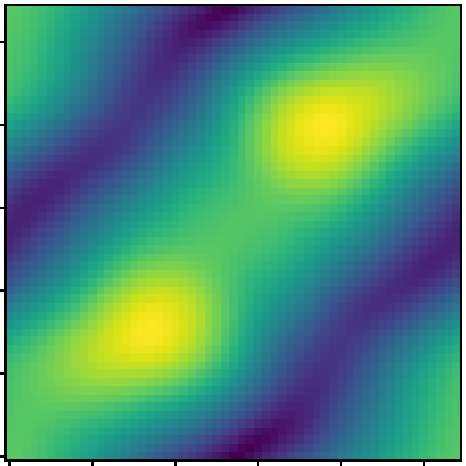
\includegraphics[scale=0.85]{figures/hsn_field.pdf}\hspace{0.5in}
%     % 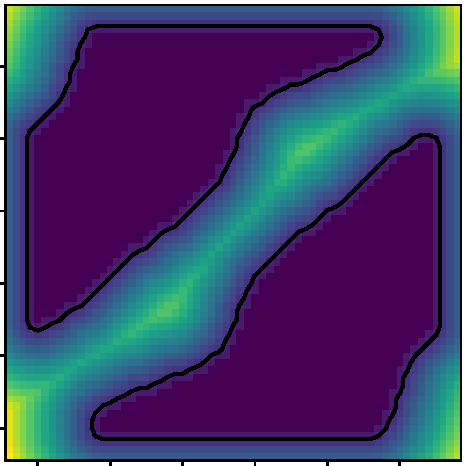
\includegraphics[scale=0.8]{figures/hsn_boundary.pdf}
%     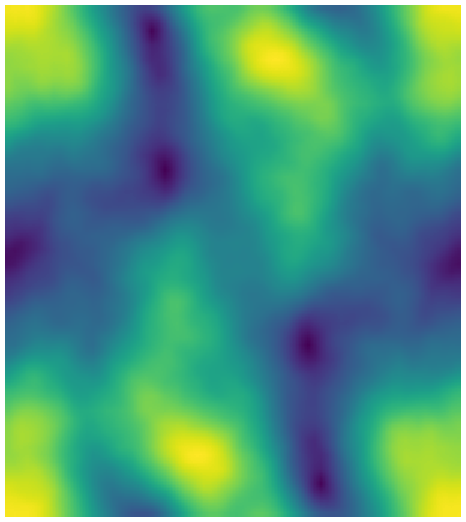
\includegraphics[scale=0.8]{figures/hsn_domain_0.pdf}\hspace{0.5in}
%     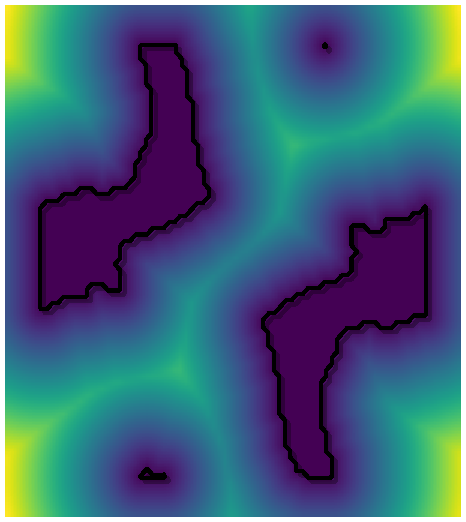
\includegraphics[scale=0.8]{figures/hsn_domain_1.pdf}
%     \caption{(Left) A gaussian random field as a function on the plane.
%             (Right) The distance to a sublevel set of the function identified as our domain $\D$ with boundary $\B$ in black.}
%     \label{fig:hsn}
% \end{figure}
%
% We then sample the domain with a collection of points $P\subset\D$ and select a subset $Q$ of $P$ within a fixed distance $\alpha$ of $\B$.
% The Dionysus C++ library~\cite{dionysus2} is used to construct the 3-dimensional rips complex of $P$ at scale $\beta = 3\alpha$ in addition to the persistent relative homology of the pair $(\rips^\beta(P), \rips^\beta(Q))$.
% The rank of the inclusion \[H_2(\rips^\alpha(P), \rips^\alpha(Q))\to H_2(\rips^\beta(P), \rips^\beta(Q))\] is identified as the number of features in $\dgm_2(\rips^\beta(P), \rips^\beta(P))$ which have not died at scale $\beta$, but were born at scale at most $\alpha$.
% This is then compared to the number of connected components in $\rips^\alpha(P\setminus Q)$ as the number of features in $\dgm_0(\rips^\alpha(P\setminus Q))$ that have not died at scale $\alpha$.
%
% \begin{figure}[htbp]
% \centering
%     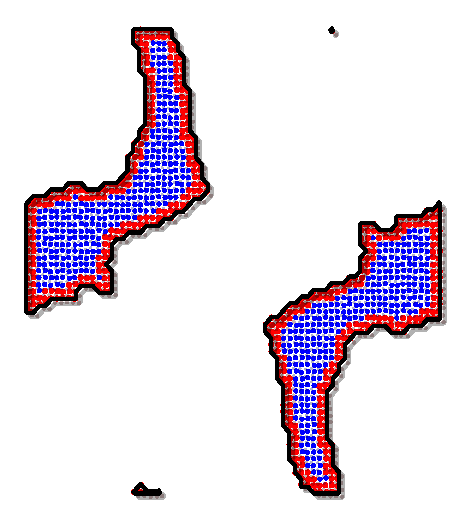
\includegraphics[scale=1.]{figures/hsn_domain_2.pdf}
%     \caption{The resulting sampled domain $P$ with $Q$ in red.}
%     \label{fig:hsn_domain}
% \end{figure}
%
% \begin{figure}[htbp]
% \centering
%     % 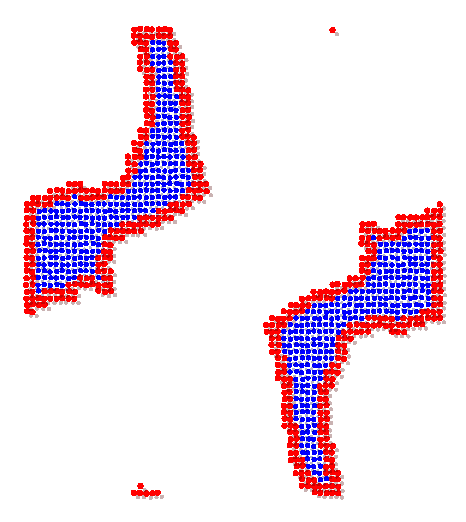
\includegraphics[scale=0.8]{figures/hsn_size_0.pdf}
%     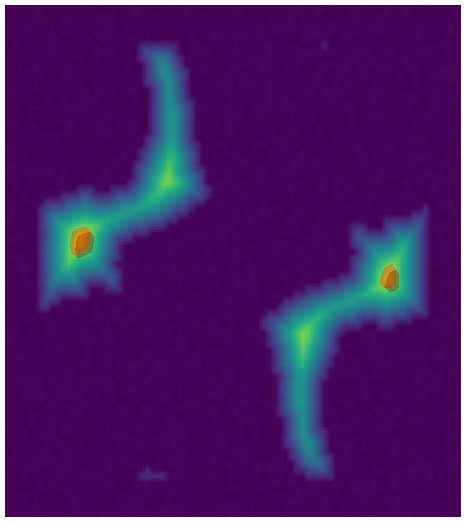
\includegraphics[scale=0.8]{figures/hsn_size_1.pdf}\hspace{0.5in}
%     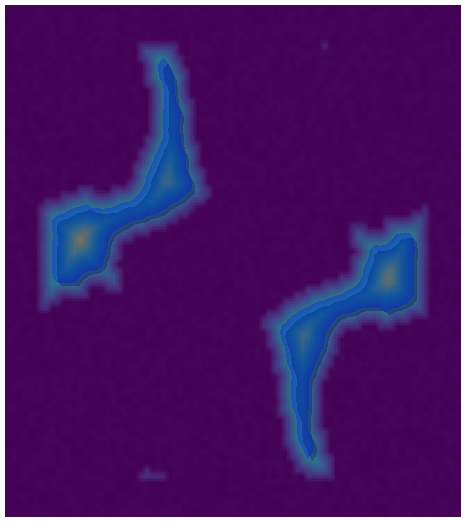
\includegraphics[scale=0.8]{figures/hsn_size_2.pdf}
%     \caption{Verification of assumption 1 via sublevel sets of the distance to the complement of $\D$:
%             $\D\setminus\B^{\alpha+\beta}$ (left) $\D\setminus\B^{2\alpha}$ (right).}
%     \label{fig:hsn_size}
% \end{figure}
%
% \begin{figure}[htbp]
% \centering
%     % 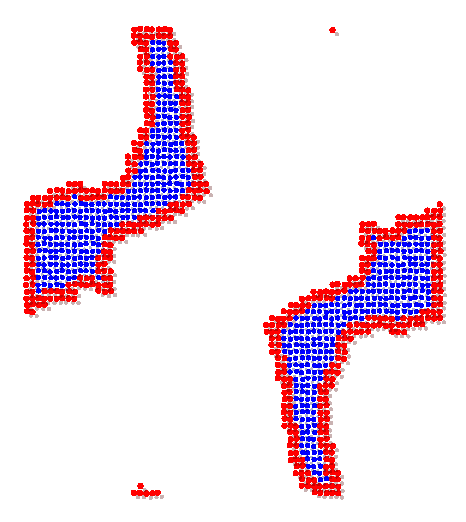
\includegraphics[scale=0.6]{figures/hsn_close_0.pdf}
%     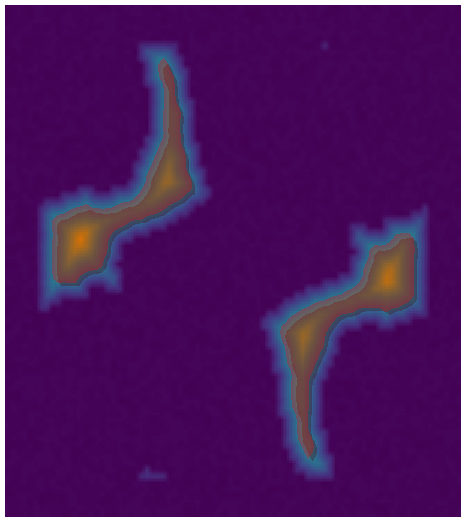
\includegraphics[scale=0.8]{figures/hsn_close_1.pdf}\hspace{0.5in}
%     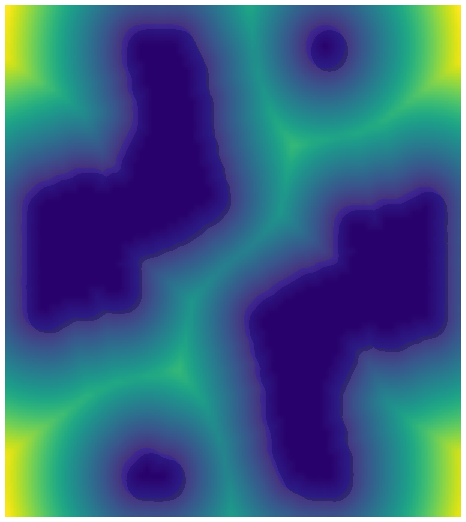
\includegraphics[scale=0.8]{figures/hsn_close_2.pdf}
%     \caption{Verification of assumption 2 via sublevel sets of the distance to the complement of $\D$ (left) and the distance to $\D\setminus\B$ (right);
%             $\D\setminus\B^{2\alpha}$ (left) $(\D\setminus\B)^{2\alpha}$ (right).}
%     \label{fig:hsn_close}
% \end{figure}
%
% \begin{figure}[htbp]
% \centering
%     % 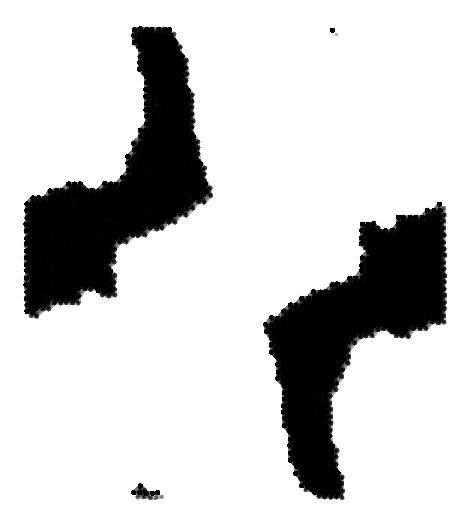
\includegraphics[scale=0.8]{figures/hsn_net_0.pdf}
%     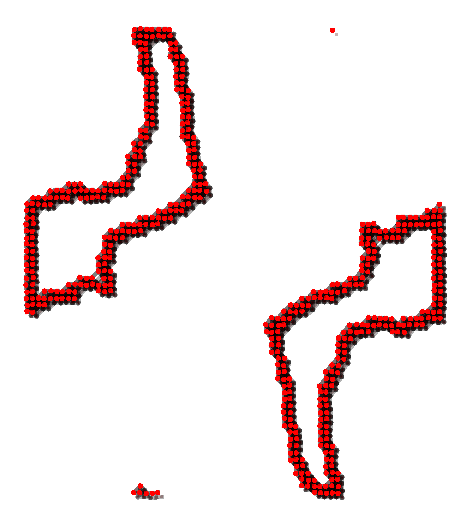
\includegraphics[scale=0.8]{figures/hsn_net_1.pdf}\hspace{0.4in}
%     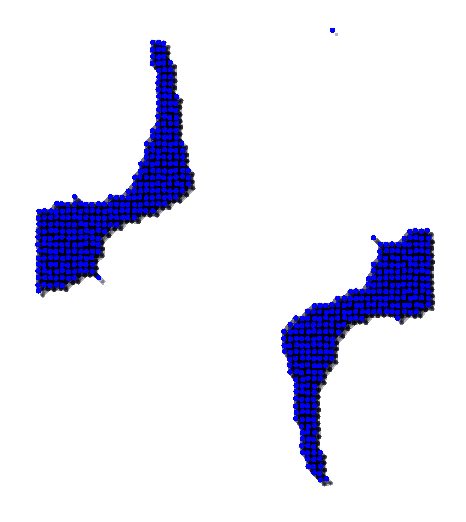
\includegraphics[scale=0.8]{figures/hsn_net_2.pdf}
%     \caption{Subcomplexes of $\rips^\alpha(P)$ restricted to $Q$ (left) and $P\setminus Q$ (right).}
%     \label{fig:hsn_net}
% \end{figure}
%
% % section tcc (end)
